
When working on a pack, I make tons of drawings. I start with the basic shape, I add the features I have in mind, I draw multiple mockup or variants of that shape, and its prominent features, then I go more into details, focusing on each features, these getting variants of their own. And so on, until I get a pretty good idea of what I want to build. You can see the final design in the illustration \ref{img:pack-side-full}.

\begin{figure}[h]
  \centering
  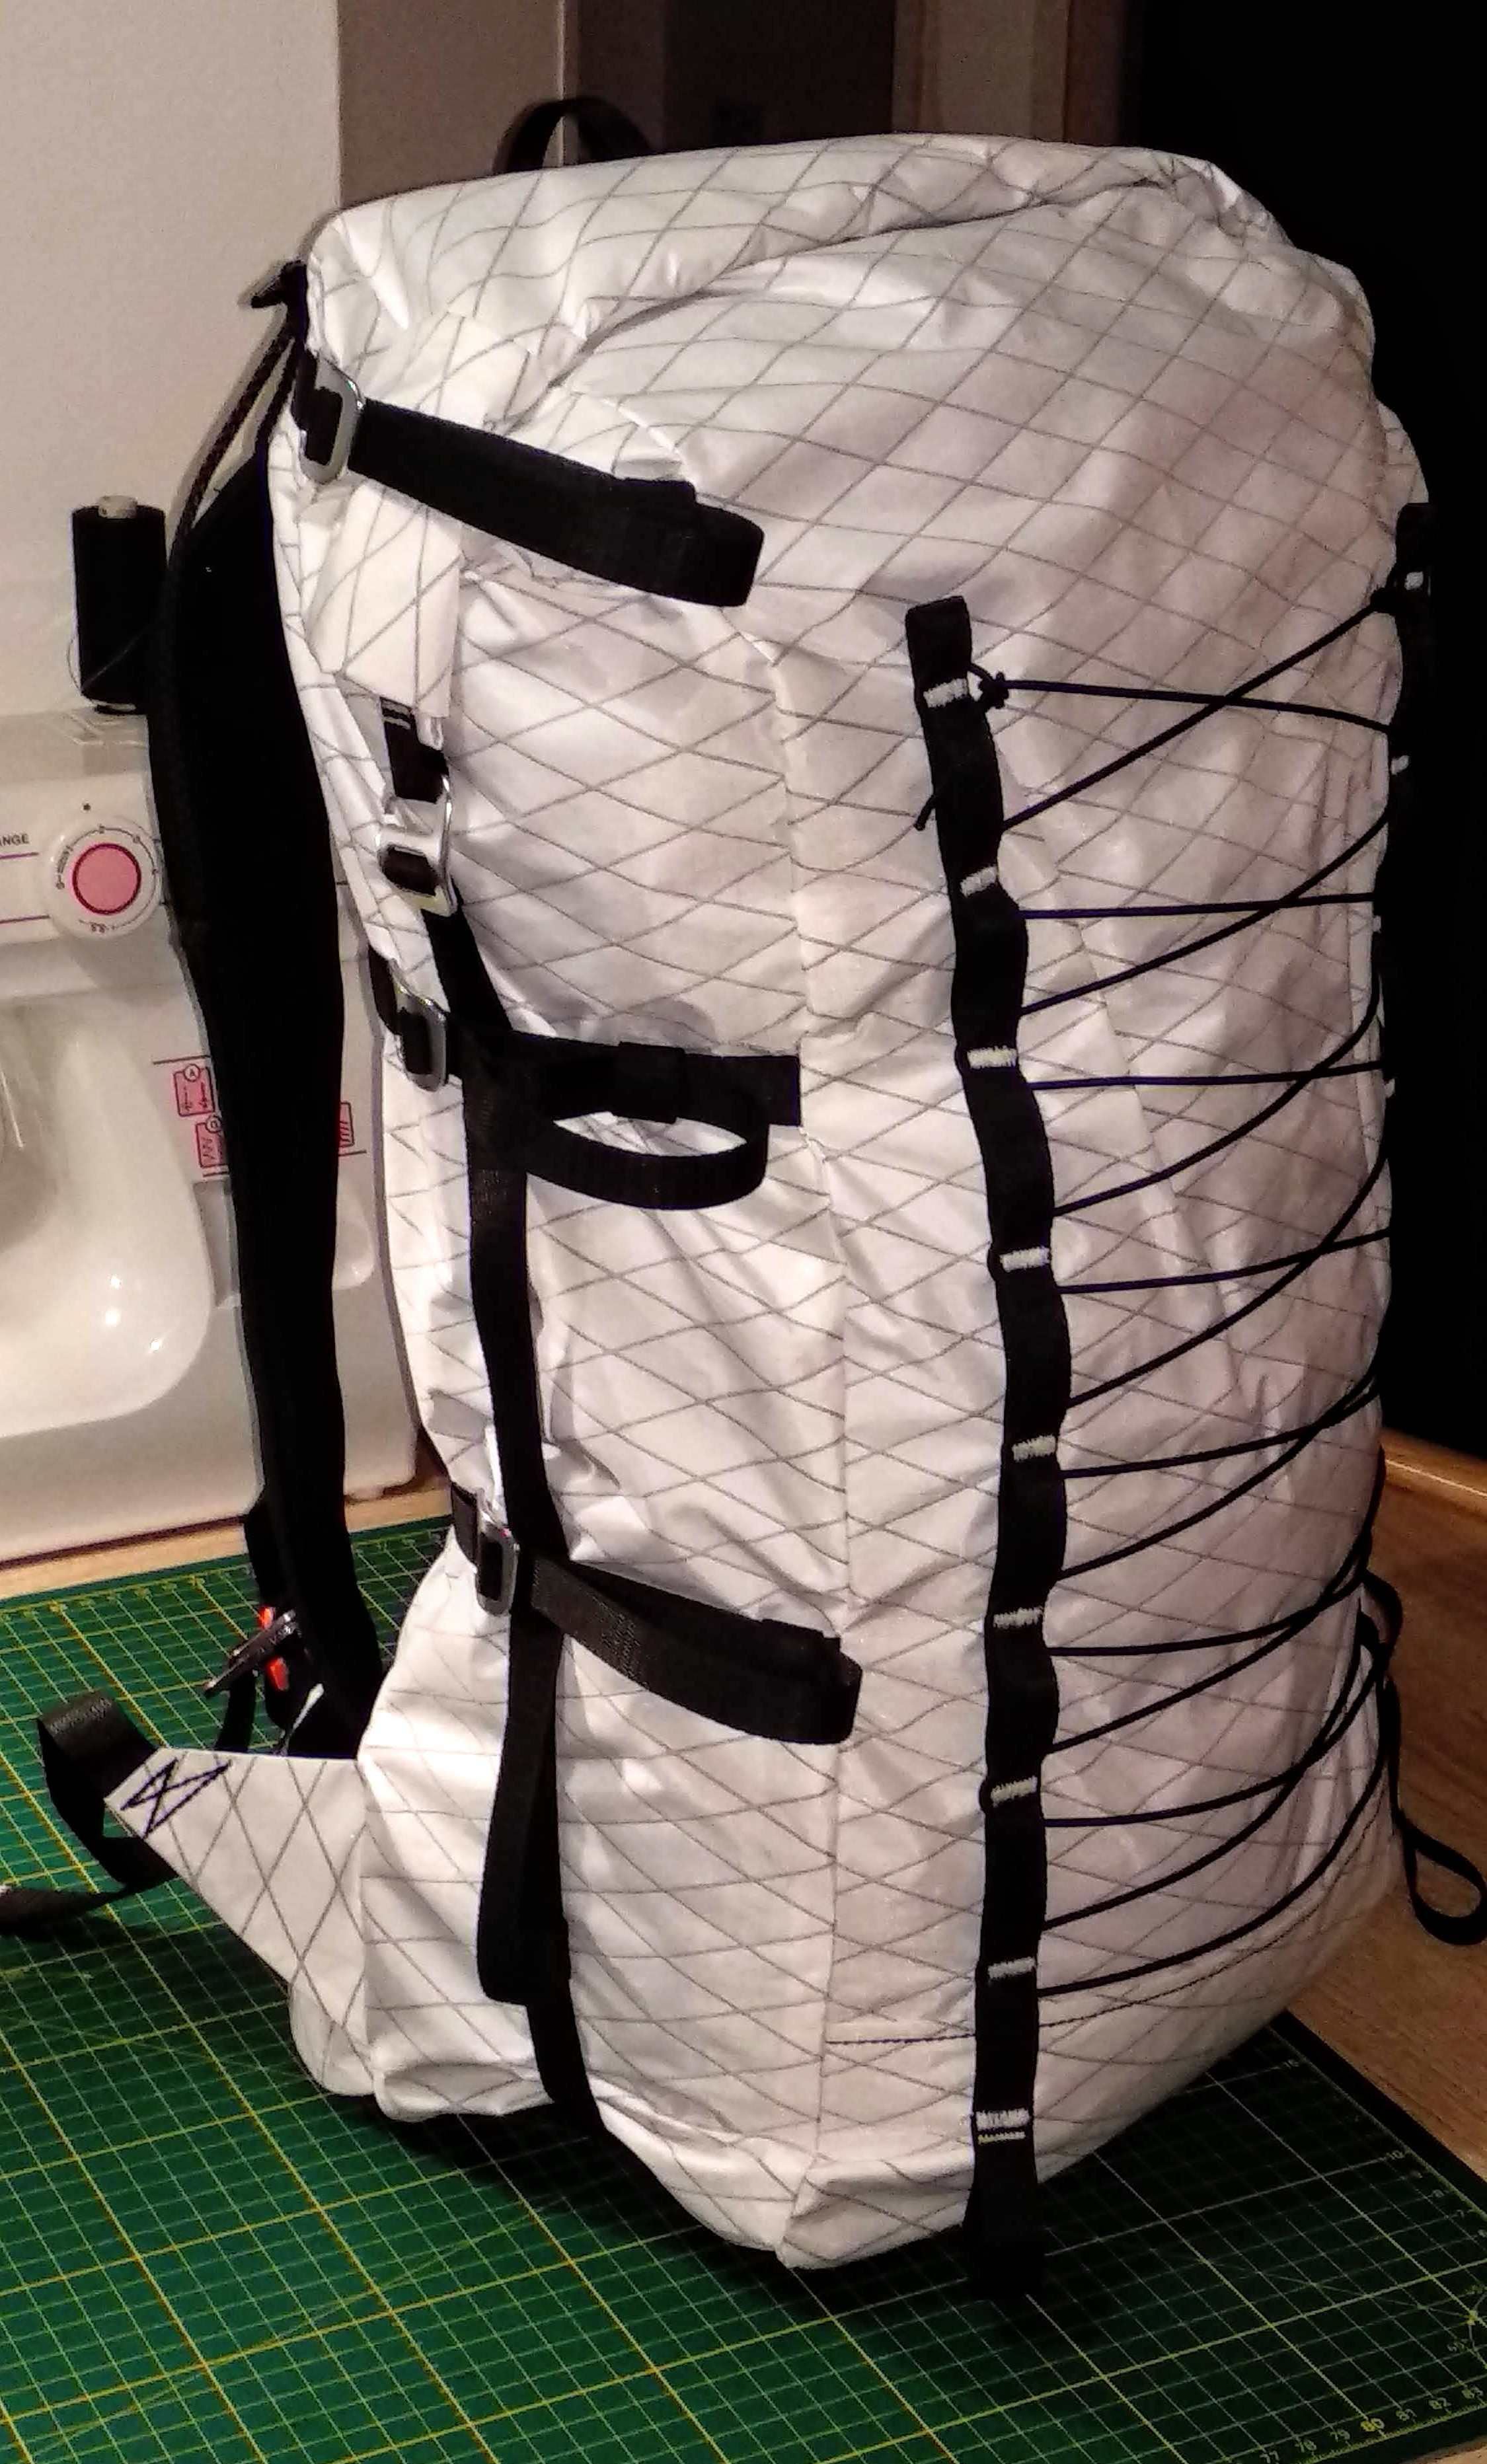
\includegraphics[width=0.5\textwidth]{media/images/pack-side-full}
  \caption{The end result of the example design in illustration \ref{img:design-drawings}}
  \label{img:pack-side-full}
\end{figure}

Let me show you an example. The illustration \ref{img:design-drawings} represents the first steps of designing a forty-ish litre hiking pack. It has no external pockets, a front interlaced elastic shock cord for drying stuff while walking, a series of 3 straps on each side of the pack for attachment and compression, and a hip belt.

\begin{figure}[h]
  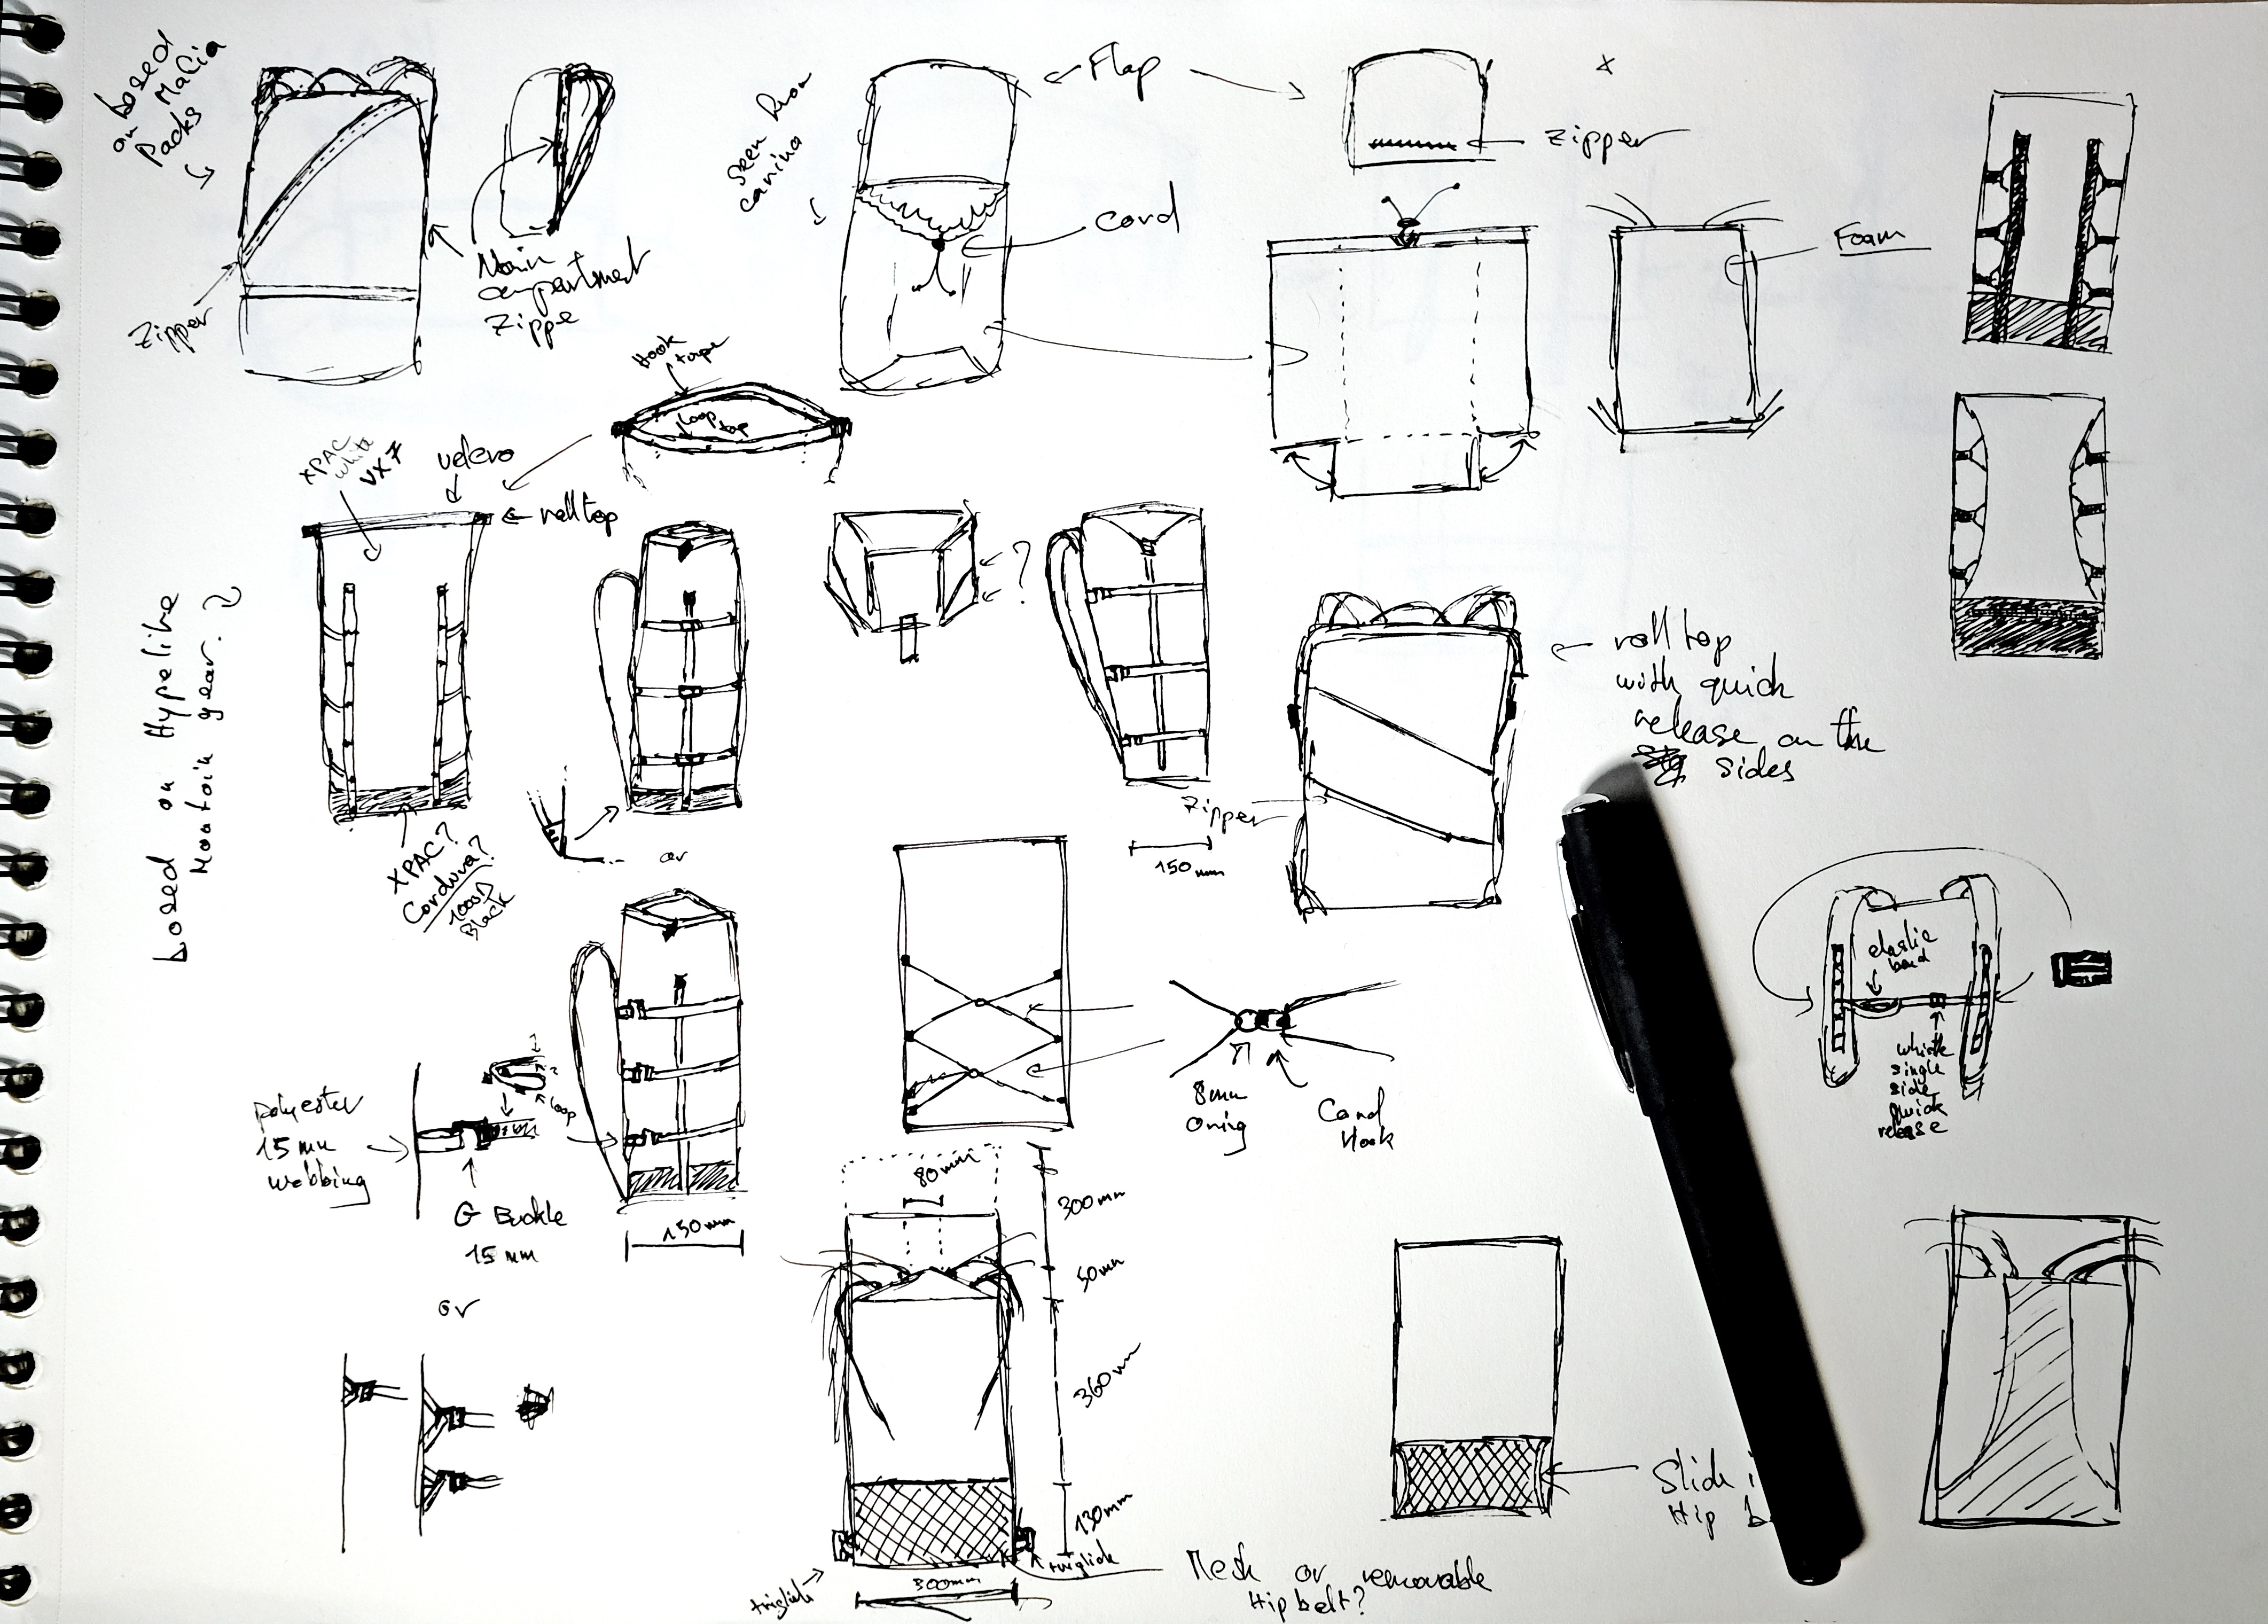
\includegraphics[width=\textwidth]{media/images/design-drawings}
  \caption{Example of drawing process (page one of many)}
  \label{img:design-drawings}
\end{figure}

\begin{figure}[h]
  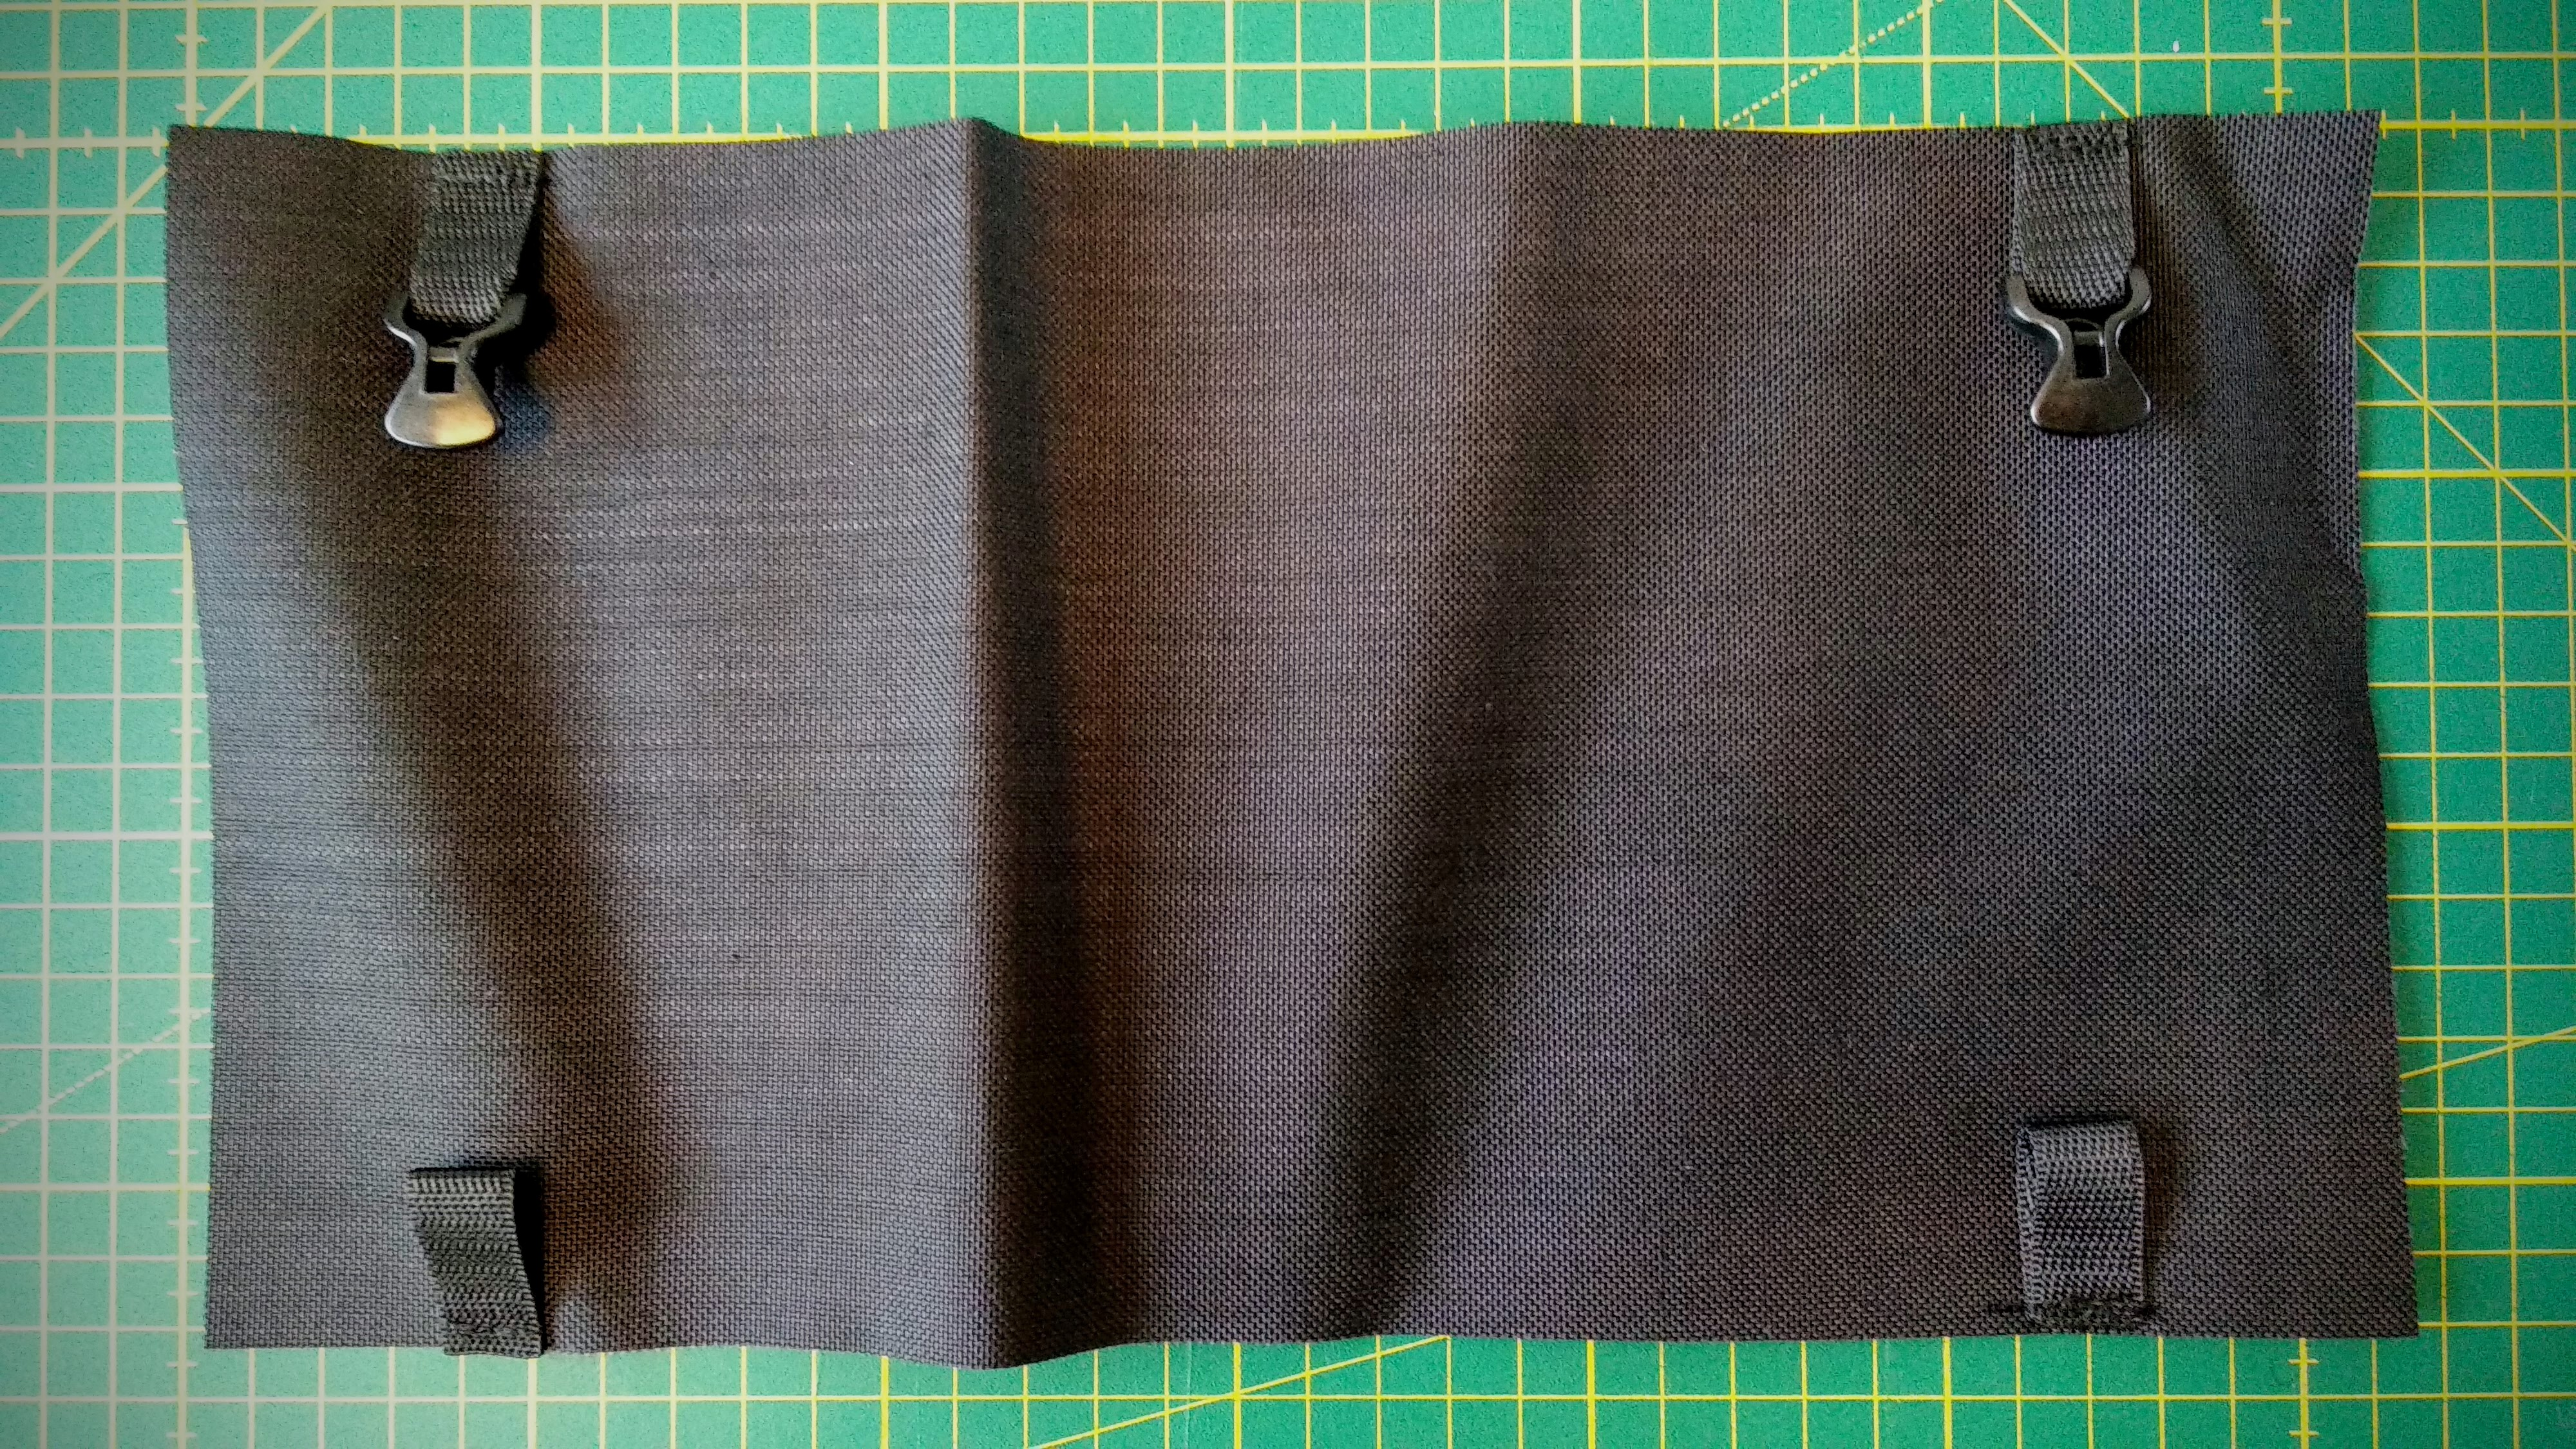
\includegraphics[width=\textwidth]{media/images/pack-bottom-cut}
  \caption{The 1000D coated Cordura bottom cut of pack shown in \ref{img:pack-side-full}}
  \label{img:pack-bottom-cut}
\end{figure}
